\chapter{基于DBpedia的语义关联度模型}
\label{chap:chap04}

本章基于DBpedia构建知识关联网络,对于其中词语与实体之间的对应关系,本文综合考虑文本外链与文章对词语的影响来计算词语与实体的关联度。在实体层,我们提出一种实体嵌入方法,综合考虑实体周围的属性信息及其所处的网络结构的拓扑信息。由此,我们可以更好地利用实体之间的语义信息计算词语之间的语义关联度。

\section{DBpedia简介}

\begin{figure}[!ht]
    \centerline{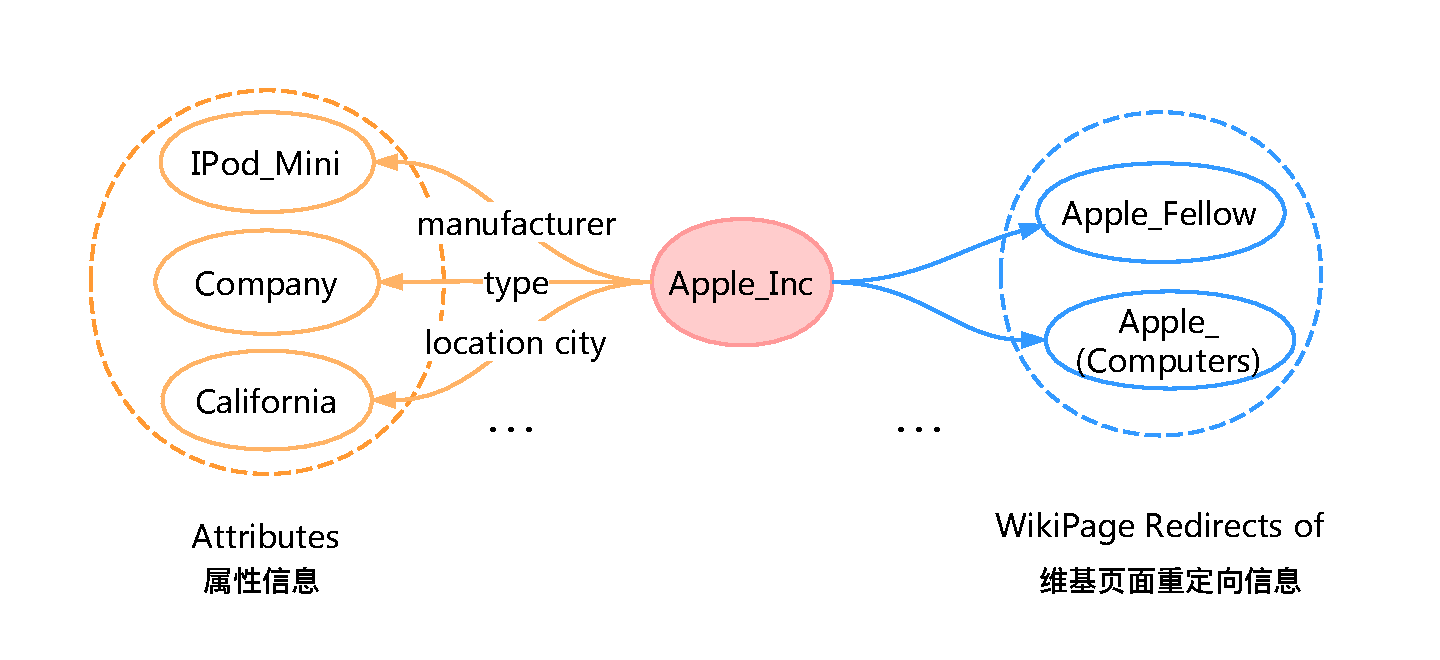
\includegraphics[width=0.9\textwidth]{chap4-1.pdf}}
    \smallcaption{DBpedia中实体的语义特征示例}
    \label{chap4-1}
\end{figure}

% 意义
DBpedia是一项由开源社区维护的百科开源知识图谱,它源自于Wikipedia又不止与此。基于万物互连的思想,DBpedia连接起了Wikipedia、Wikitionary、WordNet以及其它大型开源知识库如Yago等,不仅如此,DBpedia还提供了可供全网访问的服务,研究者们可以以DBpedia为基础挖掘到越来越多的知识信息,大大方便了各项人工智能任务的推进。

至2016年10月,DBpedia中包含了大约600万实体和13亿条RDF三元组,实体周围包含着丰富的语义信息。如图\ref{chap4-1}所示,对于科技公司\emph{Apple},其在DBpedia中有唯一的URI(统一资源定位符)表示\emph{<http://dbpedia.org/page/Apple\_Inc>},简记为\emph{Apple\_Inc},同时还有多种实体以不同关系与\emph{Apple\_Inc}相连。其中,如\emph{Apple\_Inc}是\emph{IPod\_Mini}的生产商、\emph{Apple\_Inc}是一家公司\emph{Company}以及\emph{Apple\_Inc}位于\emph{California}等等描述了该实体的属性(Attributes)空间;而另一些关系如图\ref{chap4-1}所示,不包含明确的语义信息,仅仅在语料库中与该实体通过页面重定向关系(Wikipage Redirects of)相连。

%存储
DBpedia中实体及其边的关系主要以RDF的形式存储在开源图数据库OpenLink Virtuoso\footnote{https://virtuoso.openlinksw.com/}中,并且用户可以通过Virtuoso开放的SPARQL端口\footnote{http://dbpedia.org/sparql}来通过HTTP请求访问DBpedia中的数据。其中SPARQL是一种针对RDF数据的图查询语言,能够自定模式来查询知识图谱中符合模式条件的三元组。


\section{知识关联网络构建}

\begin{figure}[!ht]
    \centerline{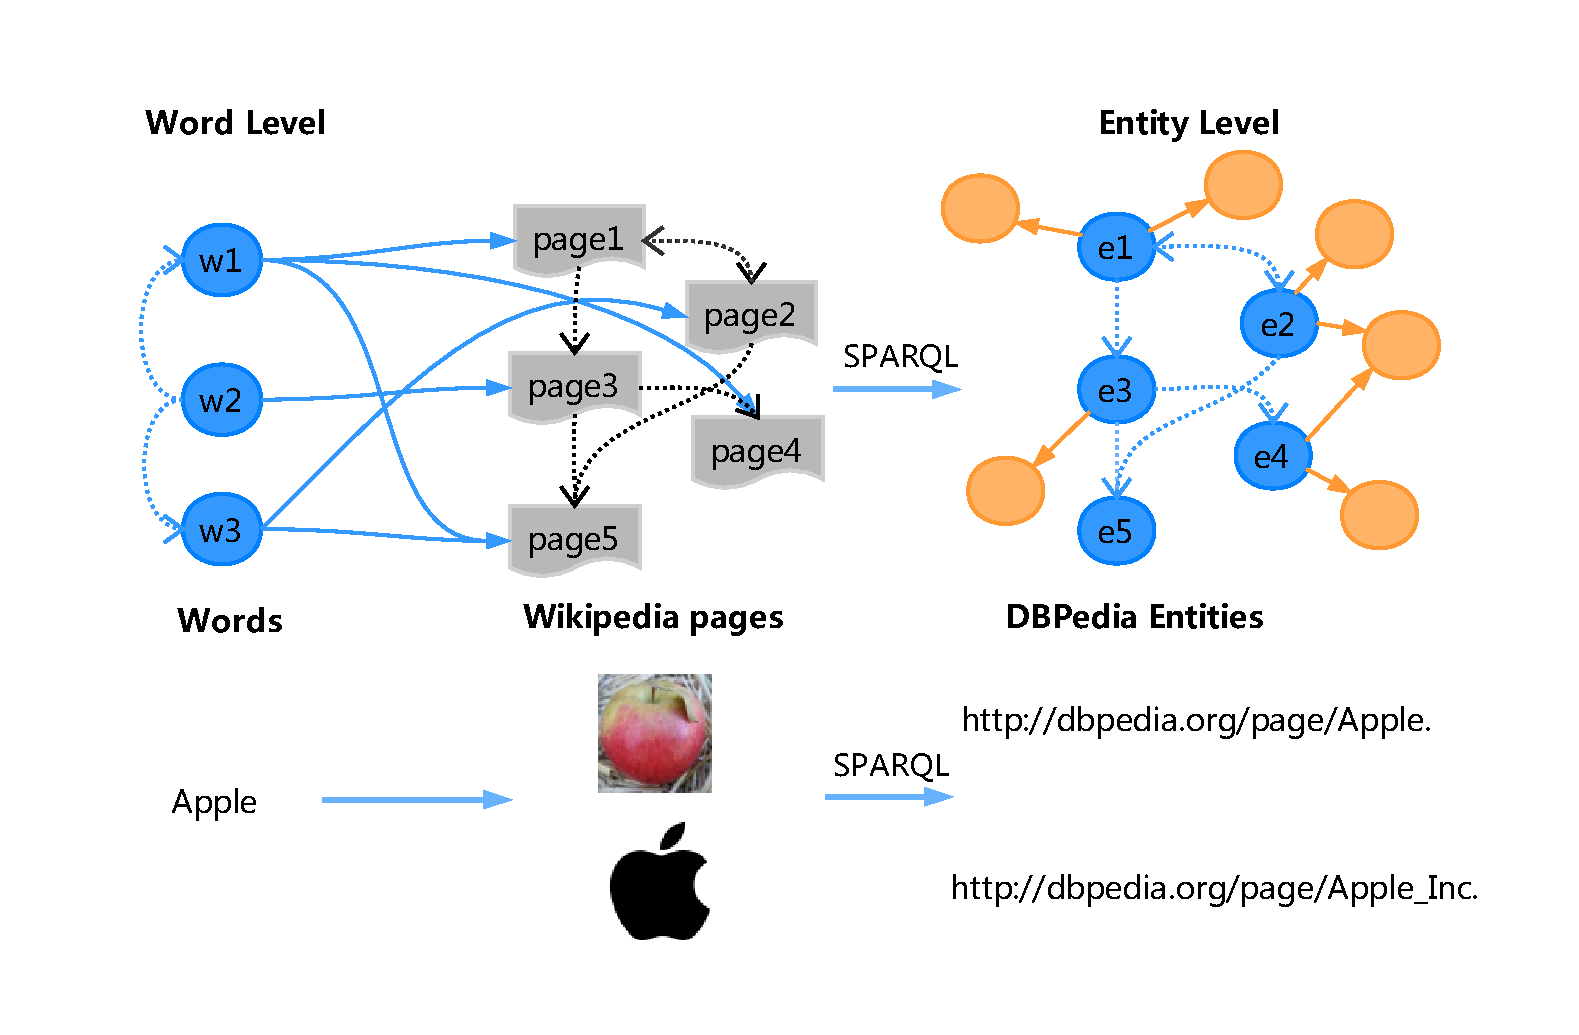
\includegraphics[width=1\textwidth]{chap4-2.pdf}}
    \smallcaption{基于DBpedia中构建的知识关联网络示例}
    \label{chap4-2}
\end{figure}

在上一章中基于WordNet构建的知识关联网络中,词语与WordNet实体之间的对应关系被人工标记并存储在WordNet中,可以很方便地被查询到。与之不同的是,我们无法直接拿到词语与DBpedia实体的关系。但是语料库Wikipedia中则包含了丰富的词语,其文本由词语构成,分类信息、外链信息等也都自然地表现为文本。而且Wikipedia中的页面也与DBpedia中的实体一一对应。文本基于这种对应关系,通过Wikipedia建立其词语与DBpedia中实体的对应关系。

如图\ref{chap4-2}所示,我们给出了基于DBpedia构建知识关联网络的例子。对于一个给定的单词$apple$,通过TF-IDF或词频统计等文本分析手段,我们可以得到与之相关的维基页面,比如维基百科中描述一种水果的$Apple$页面和描述一家公司的$Apple\_Inc$页面,其中每个维基页面有一个重要的属性叫做\emph{WikiPageId},形式上表现为数字,唯一地标示了Wikipedia中的一篇文章。这个属性在DBpedia中也作为对应实体的属性存在。因此我们可以通过SPARQL查询到对应的DBpedia实体。举个例子来说,描述一种水果的$Apple$页面的\emph{WikiPageId}的值是$856$,我们可以通过如下的查询语言得到对应的DBpedia实体。

\begin{lstlisting}[basicstyle=\fontsize{10}{11}\ttfamily,aboveskip=1em,frame=shadowbox]
    PREFIX dbo: <http://dbpedia.org/ontology/>
    SELECT ?E WHERE {
        ?E dbo:wikiPageID 856.
    }
\end{lstlisting}

对于DBpedia中实体周围的语义信息,本文将其分为属性信息(图\ref{chap4-2}中橘色节点所示)和拓扑结构信息,其中属性信息如上节中图\ref{chap4-1}所示明确地描述了实体的属性,而拓扑结构信息反映了实体之间的结构信息。在本文中为了更方便地表示实体的属性与拓扑结构空间,我们将实体属性所构成的图表示为$G_{attr} = \{a_1, a_2, ..., a_n\}$, 其中每个$a_i$描述了一条关系,这段关系以三元组的形式表现,由头实体(h)、关系(r)和尾实体(t)构成,即$a_i = (h, r, t)$。而对于实体所处的拓扑结构,我们将其定义为$G_{t} = (E, R_{redirect})$,表示由边$R_{redirect}$即\emph{WikiPageRedirectOf}连接的所有实体集$E$所构成的图。由此我们可以应用网络嵌入模型来学习实体的属性空间与拓扑结构空间的向量表示。

\section{语义关联度计算}
如图\ref{chap4-3}所示,我们给出了基于DBpedia中构建的知识关联网络驱动的语义关联度计算流程,图中实线表示了模型的处理流程,而虚线表示了一种将输入部分转化为输出部分的处理方法。可见我们的模型主要包含下面三个部分:1)经过对Wikipedia的简单预处理,我们得到词语与维基百科页面的对应关系;2)由维基页面唯一的\emph{id},经过SPARQL查询得到维基页面对应的DBPedia实体,连接起词语与实体的对应关系;3)对于知识关联网络实体层的语义信息,我们将其分为属性空间与拓扑结构空间,并采用不同的网络嵌入模型去得到实体的向量表示。最后,我们综合考虑词语与词语、词语与实体以及实体与实体之间的语义关联度去构成最后的关联度度量。

\begin{figure}[!ht]
    \centerline{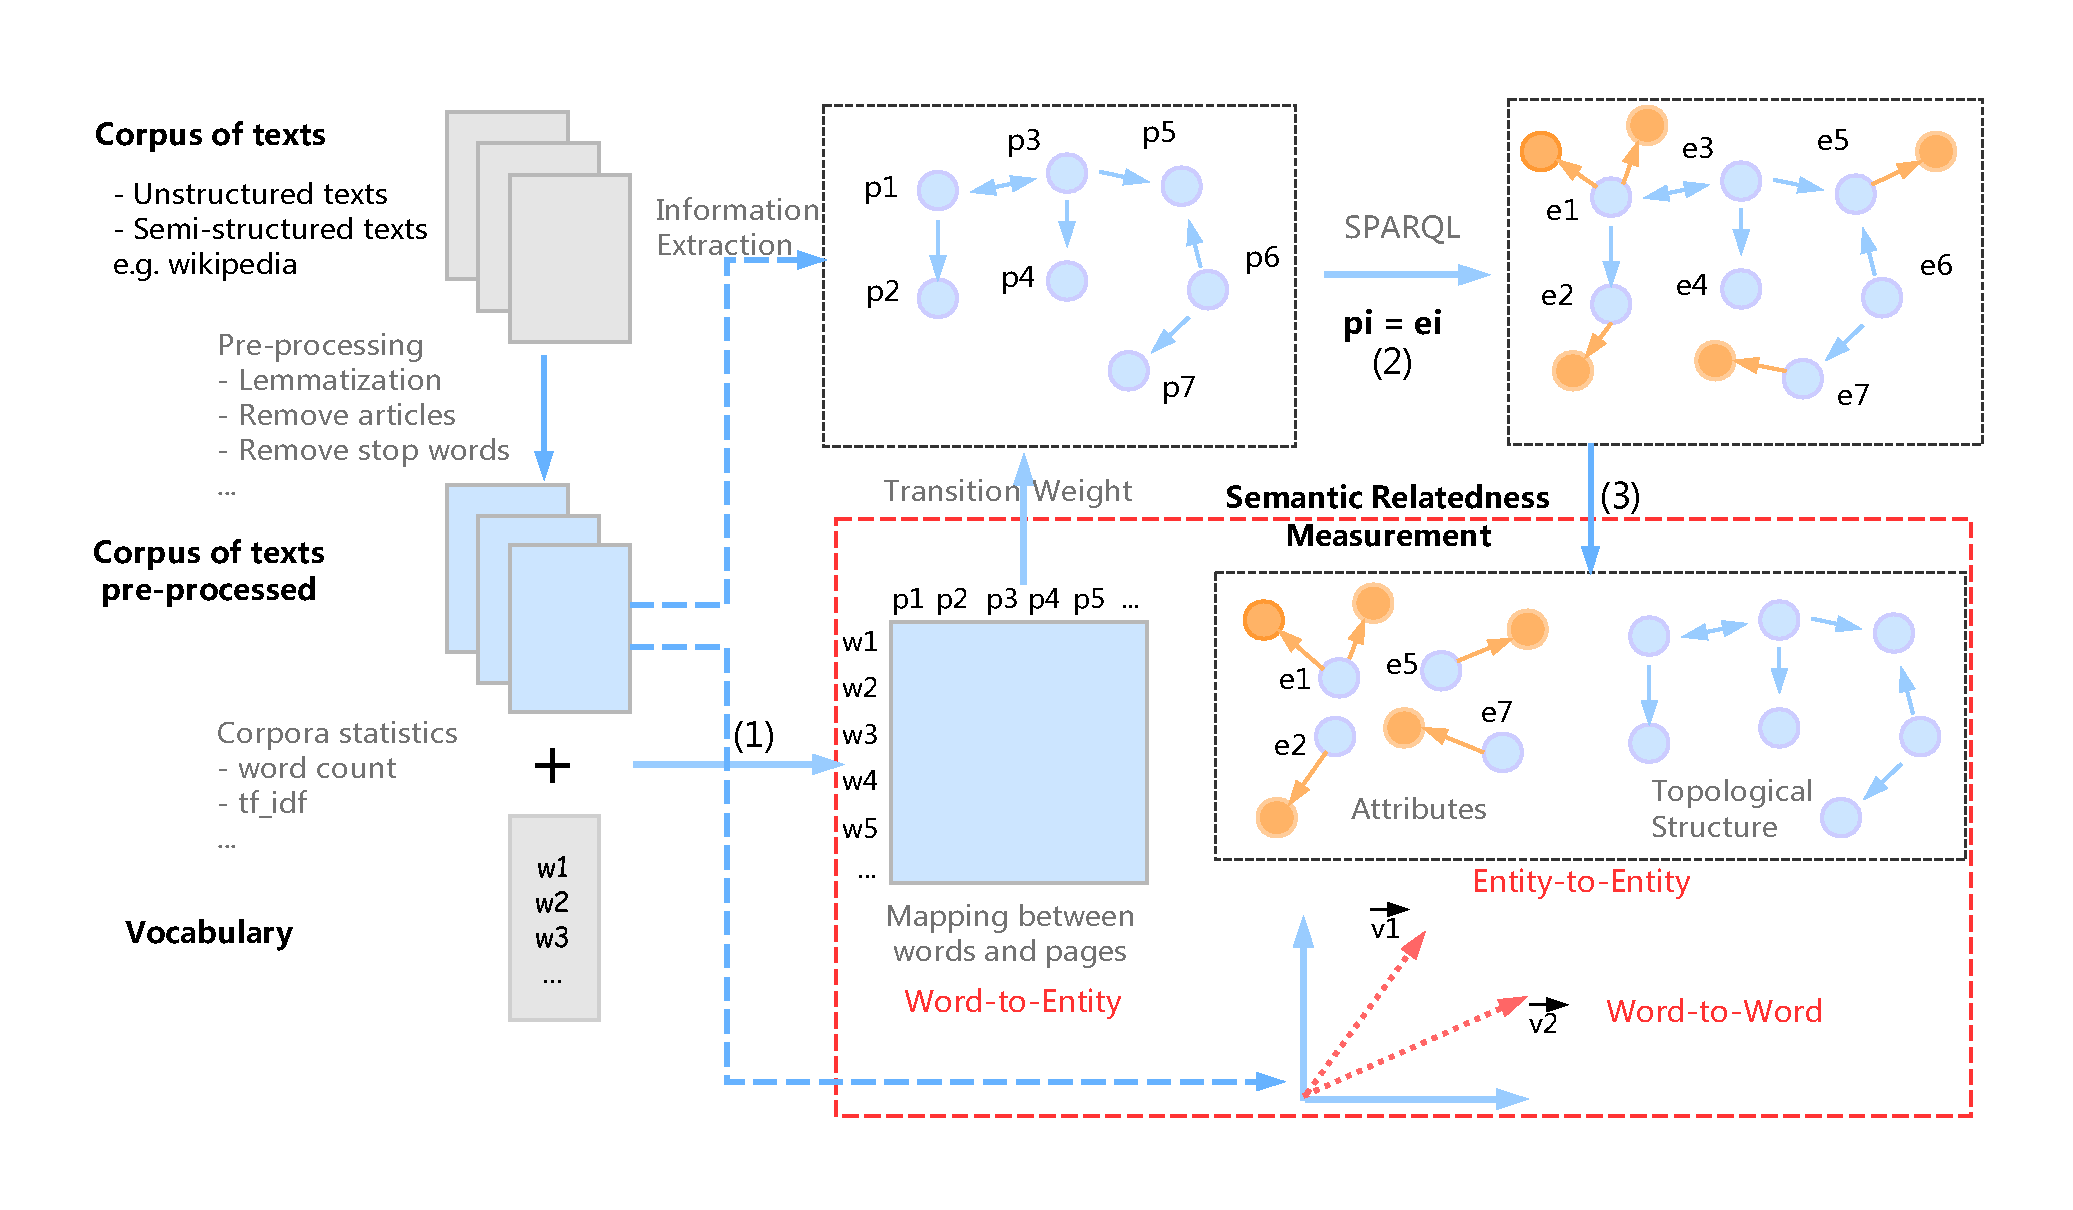
\includegraphics[width=1\textwidth]{chap4-3.pdf}}
    \smallcaption{基于DBpedia中构建的知识关联网络驱动的语义关联度计算流程}
    \label{chap4-3}
\end{figure}

\subsection{词语之间的语义关联度计算}
\label{dbpedia_word2vec}
这部分的处理同本文\ref{word2vec},本节不做赘述。

\subsection{词语与实体之间的的语义关联度计算}
在知识关联网络中,词语层与实体层之间存在着多对多的关系。由于词语的多义性,对于一个给定的词,知识关联网络中存在着多个实体与之对应。为了计算一个词语($w$)与一个实体($e$)之间的关联度,1)一些研究者们将词语与实体之间的共现次数作为其关联度标准~\cite{aaai/Pirro12},但是这种方法对于一些频次较高的常用词不敏感,如\emph{this}、\emph{that}等。2)还有一些研究者从词语的意义角度出发~\cite{aaai/GongXH18},他们认为如果实体$e$是词语$w$的唯一关联实体,则$e$和$w$高度相关联。基于这种假设他们通过链接受欢迎度(Link Popularity,LP)来计算强相关的锚文本词语与其对应的实体之间的关联度:
\begin{equation}
    \label{lp}
    LP(w, e) = \sum_{P}^{ }\sum_{S \in P, w \in S}^{ } \frac{\sum_{w^{'} \in S}^{ }tf\_idf(w^{'},e)}
    {\sum_{e^{'} \in e(w)}^{ }\sum_{w^{'} \in S}^{ }tf\_idf(w^{'}, e^{'})}
\end{equation}
\noindent 其中,$P$代表维基百科的一篇文章,$S$代表$P$中包含词语$w$的句子,$w^{'}$则表示组成句子$S$的词语。$e(w)$表示有锚文本单词$w$外链指向的所有页面集合,即实体集合。这种方法仅仅考虑来锚文本词语与外链页面的关系,忽略了词语与包含该词语的当前页面的关系,本文扩展$e(w)$为:
\begin{equation}
    \label{entities-set}
    e(w) = e_{a}(w) \cup e_{m}(w)
\end{equation}
\noindent 其中$e_{a}(w)$代表了公式\ref{lp} 中的由锚文本指向的实体集合,而$e_{m}(w)$指包含该词的且不是该词对应锚文本指向的实体页面。然后我们提出全受欢迎度(Full Popularity, FP)来计算词语与实体之间的关联度,有:
\begin{equation}
    \label{fp}
    FP(w,e) = \left\{\begin{matrix}
        LP(w,e) & e \in e_{a}(w) & \\
        \frac{tf\_idf(w,e)}{\sum_{e^{'} \in e_m(w)}^{ }tf\_idf(w,e^{'})} & e \in e_{m}(w) & 
        \end{matrix}\right.
\end{equation}
\noindent 最后对于一个词语$w$与实体$e$之间的关联度,有:
\begin{equation}
    \label{f_we}
    f_{we}(w, e) = \frac{FP(w, e)}{\sum_{e^{'} \in e(w)}^{ }FP(w, e^{'})}
\end{equation}


\subsection{实体之间的语义关联度计算}
\label{subsec4-3-3}
知识关联网络的实体层本质上表现为多关系图,其中实体的语义信息同时被实体周围的属性信息,以及实体所处的网络拓扑结构所描述。属性信息部分描述了细致的语义关系如A是B的朋友,B是组织C的成员等,而拓扑结构信息则反映了实体间的共现信息中的潜在语义信息。两个实体可能拥有完全不同的属性空间描述,但他们处在相似的网络空间结构中,同样地两个处在不同结构中的实体可能拥有相同的属性空间。在本节提出的模型中,我们采取两种不同的模型分别学习实体在属性空间与拓扑结构空间的分布式向量表示,最后通过加权求和的方式得到实体之间的语义关联度。

\textbf{属性空间嵌入:}对于属性空间的嵌入,最简单直接的方法是\emph{one-hot}编码。这种方法枚举所有属性类型,然后生成一个长度等于属性类型总量的向量,向量中每个元素对应于一个属性。这样对于一个实体的属性空间来说,其拥有的属性对应的向量元素为1,没有的的属性为0,每个实体最后对应的向量长度都等于属性总量。对于DBpedia来说其属性类型总量是百万量级的,\emph{one-hot}编码消耗巨大且效果不好。

对于知识图谱中三元组所描述的明确语义信息,之前很多研究者们将头实体(h)、关系(r)和尾实体(t)这样的关系映射到低维向量空间上的转移操作,认为其对应的向量表示满足下面的关系~\cite{nips/BordesUGWY13, aaai/WuFCABW18}:
\begin{equation}
    \label{hrt}
    \vec h + \vec r \approx \vec t
\end{equation}

\noindent 基于这样的理论,本文将实体属性向量空间表示为$\mathbb{R_a} ^ {N \times d}$,其中假设$N$代表着所有属性实体总量,$d$表示为实体在属性空间的向量维度。我们结合实体以及关系来最小化Margin Ranking损失,即通过最小化正例实体属性对之间间隔,最大化负例实体属性对之间间隔这样的方法来学习其向量表示:
\begin{equation}
    \label{attribute_formula}
    \mathcal{L} = \sum_{(a,b) \in G_{attr}^+}^{ } \sum_{b^- \in G_{attr}^-}^{ }[\ell + cos(a,b)-cos(a,b^-)]_+
\end{equation}

\noindent 公式中$[x]_+=max(0, x)$,$\ell$代表间隔超参数。$G_{attr}$表示由多组\emph{(h, r, t)}三元祖构成的图属性空间,公式中$G_{attr}^+$表示正例三元组构成的图属性空间,$G_{attr}^-$表示负例三元组构成的图属性空间。其中,我们通过下面两种采样策略去得到$G_{attr}^+$:1)正例$a$由头实体h和关系r共同构成,而正例$b$仅包含尾实体t;2)正例$a$仅包含头实体h,正例$b$包含关系r和尾实体t。至于$b^-$则$G_{attr}^-$中表示采样到的负样例,本文采用k-负采样策略~\cite{corr/Mikolov13}在每个批次(batch)更新中去得到k个负样例对。最后我们采用随机梯度下降法(stochastic gradient descent,SGD)去优化公式\ref{attribute_formula}。值得注意的是,每次SGD更新参数的步骤发生在$G_{attr}^+$采样正例并求损失之后。

\textbf{拓扑结构空间嵌入:}
一个实体的拓扑结构空间包含着描述这个实体的潜在语义信息,举个例子来说,当某用户在浏览器中访问到\emph{Apple\_Inc}这个页面时,页面中包含着大量的该用户可能感兴趣的描述其他实体的页面,像\emph{Microsoft\_Windows}或者\emph{Graphical user interface},但是这些实体并不是\emph{Apple\_Inc}的属性实体。为了去考虑这样的隐含信息,之前有很有研究者~\cite{aaai/ZhangZH15, aaai/GongXH18}尝试在Wikipedia语料库中通过文本处理去得到实体间链接这样的语义特征。知识图谱DBpedia中的实体通过关系\emph{WikiPageRedirectOf}被连接,这种关系对应着Wikipedia中页面之间的链接信息。我们记这样的拓扑结构空间为$G_t = G(E, R_{redirect})$,其中$E$代表DBpedia实体集,而$R_{redirect}$代表着由\emph{WikiPageRedirectOf}构成的边集。

显而易见,$G_t$本质上表现为加权图的形式,$R_{redirect}$中的边拥有不同的转移概率。举个例子来说,某用户正在浏览器中浏览Wikipedia的一篇文章\emph{Apple\_Inc},页面中包含着其他几十个相关的文章描述了不同的实体。当该用户想要去了解更多关于{Apple\_Inc}的扩展细节时,该用户一般会首先关注到跟当前页面密切相关的文章。因此,他将会访问相关的Wikipedia页面而忽略掉相关度不高的。由此可见\emph{Apple\_Inc}与其他文章描述的实体间有不同的转移概率,而且这种转移是有方向的,即从A页面到B页面的转移概率和从B页面到A页面的转移概率可能是不同的。

然而,在DBpedia中以三元组存储的关系是无权重的。假定两个实体$e_i$和$e_j$通过关系$r_{ij}$连接,为了给关系$r_{ij}$分配权重,最简单直接的方法是考虑实体$e_i$与$e_j$对应的锚文本之间的共现关系。对于给定实体$e_j$对应的锚文本,我们记为$t_j$,使$cnt(e_i, e_j)$表示实体$e_i$对应的Wikipedia文章中文本$t_j$出现的次数,则基于计数统计的实体间$e_i$和$e_j$转移概率$W_{cnt}(e_i, e_j)$为:
\begin{equation}
    \label{cng_formula}
    W_{cnt}(e_i, e_j) = \frac{cnt(e_i, e_j)}{\sum_{e^{'} \in P_i}^{ }cnt(e_i, e^{'})}
\end{equation}

\noindent 其中$P_i$表示实体$e_i$对应的维基页面,$e^{'}$则是$P_i$中的外链锚文本指向的维基页面描述的实体。然而仅仅考虑锚文本的频率会给予很多高频词更好的权重,然而其与本实体关联度并不高。为了弥补这样的缺点,我们计算$t_j$相对于页面$P_i$的TF-IDF(Term Frequency–Inverse Document Frequency)值作为实体$e_i$到$e_j$转移概率:
\begin{equation}
    \label{w_tf-idf_formula}
    W_{tf\_idf}(e_i, e_j) = \frac{tf\_idf(e_i, e_j)}{\sum_{e^{'} \in P_i}^{ }tf\_idf(e_i, e^{'})}
\end{equation}



经过上述的步骤,我们可以得到加权图$G_t$,为了使图中实体在其拓扑结构空间中是可以比较的,我们需要将其嵌入在更具表达力的低维向量空间。在$G_t$中,拥有相似邻居的节点往往在语义空间中更加接近。本文基于这样的假设来学习实体的向量表征,对于一个实体这需要最大化其邻居节点的观测概率。形式化地说,对于一个给定的实体$e_i$,其邻居节点$(e_0, e_1, ..., e_i, ...e_l)$的观测概率可以表示为条件概率$Pr$:
\begin{equation}
    \label{pr}
    Pr((e_0, e_1, ..., e_{i-1}, e_{i+1}, ..., e_l)|e_i)
\end{equation}

\noindent 之前研究者们已经提出过多种在网络中通过随机游走生成采样序列的方法~\cite{kdd/Perozzi14, kdd/GroverL16},其中node2vec~\cite{kdd/GroverL16}中提出的偏置随机游走通过综合考虑深度优先遍历与广度优先遍历取得了不错的效果,本文也采用这种方法来生成采样序列,并基于下面的策略来进行随机游走:
\begin{equation}
    \label{zeta}
    \zeta_{pq}(t,x) = \left\{\begin{matrix}
        \frac{1}{p} && \text{if} & d_{tx} = 0 & \\
        1           && \text{if} & d_{tx} = 1 & \\
        \frac{1}{q} && \text{if} & d_{tx} = 2 & 
        \end{matrix}\right.
\end{equation} 
\noindent 其中$t$表示上次访问的节点,$x$代表下一个要访问的节点,$d_{tx}$表示节点$t$与节点$x$之间的距离,参数$p$和$q$是两个需要提前设置的参数,用来调控深度优先遍历与广度优先遍历对采样过程的影响。

如图\ref{chap4-4} 所示,对于给定的DBpedia无权图,我们通过上述基于TF-IDF的方法给图中节点之间的关系加权,然后通过公式\ref{zeta}中的偏置随机游走策略生成采样序列。图\ref{chap4-4}右侧子图展示了偏置随机游走的过程,假设我们经过红色节点$t$到达了蓝色节点$v$,接下来可能走向的节点包含$\{t, x_1, x_2\}$,根据节点$t$到到这些节点的距离,对应的偏置权重如图所示,对于$x_1$来说,$d_{tx_1}$的值为2,则$x_1$作为随机游走的下一个节点的概率为边的的权重乘上$1/q$,其他节点类似。

\begin{figure}[!ht]
    \centerline{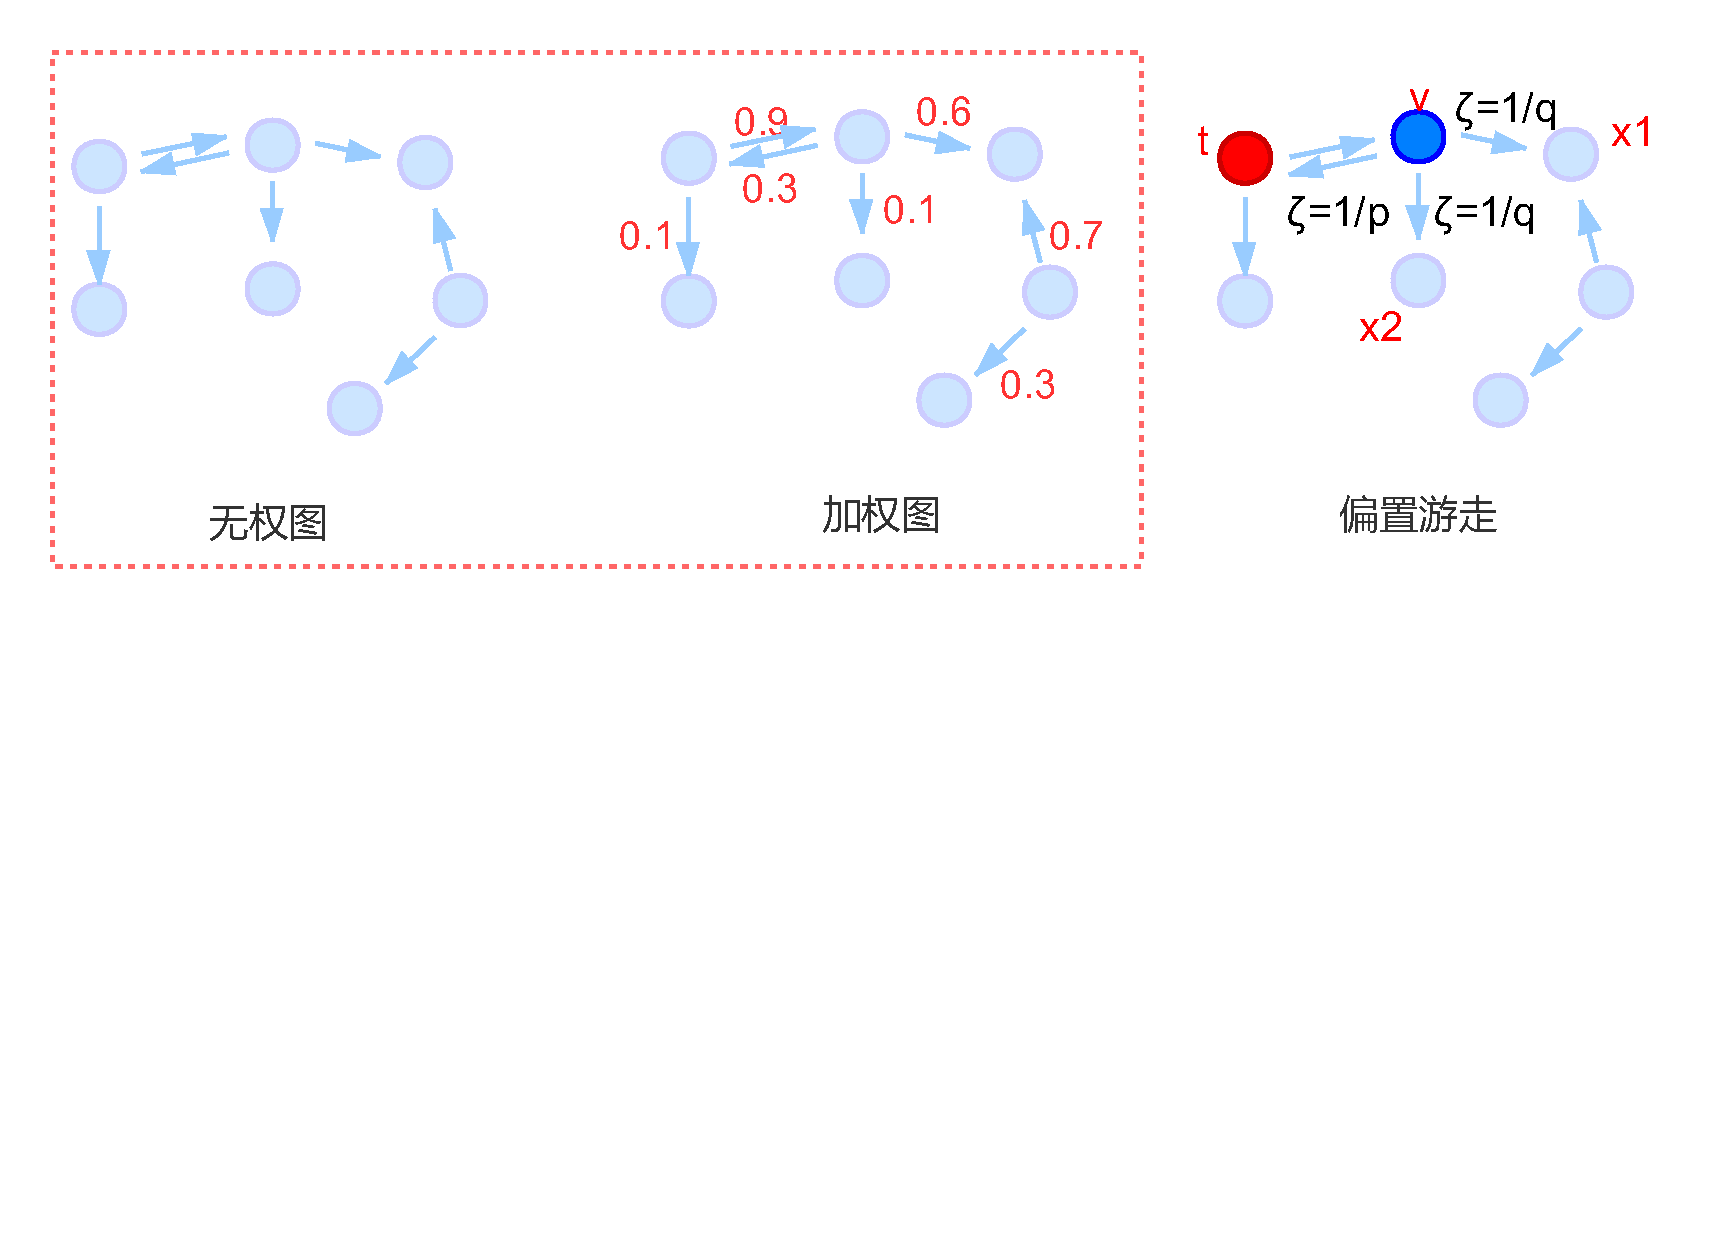
\includegraphics[width=1\textwidth]{chap4-4.pdf}}
    \smallcaption{加权图与随机游走采样示例}
    \label{chap4-4}
\end{figure}

当得到采样序列后,我们的目标是在向量空间最大化给定节点在序列中的邻居节点的观测概率,即最大化公式\ref{pr}。我们给出一个将实体映射到向量空间的函数:$\Phi: e \in E \rightarrow \mathbb{R_t}^{\left | E \right | \times d}$。其中$E$是图$G_t$中包含的所有实体,$\Phi$是一个$\left | E \right | \times d$规模的可训练的矩阵参数。通过这样的映射关系,对于$E$中每一个实体$e_i$,我们通过最小化下面的损失函数可以得到一个d维的向量,
\begin{equation}
    \label{log_pr}
    minimize\ -log Pr(N(e_i)|\Phi(e_i)) = -log\prod_{e^{'} \in N(e_i)}^{ }Pr(e^{'}|\Phi(e_i))
\end{equation}

\noindent 其中$Pr(e^{'}|\Phi(e_i))$表示在目标向量空间中实体$e^{'}$作为$e_i$出现的概率。对于$e_i$邻居$N(e_i)$中的每一个实体$e^{'}$,我们通过\emph{softmax}函数对其进行归一化处理可以得到:
\begin{equation}
    Pr(e^{'}|\Phi(e_i)) = \frac{exp(\Phi(e^{'})\cdot \Phi(e_i))}{\sum_{e_k \in N(e_i)}^{ }exp(\Phi(e_k)\cdot \Phi(e_i))}
\end{equation}
\noindent 对于实体拓扑空间的嵌入,我们通过随机梯度下降法来优化公式\ref{log_pr}。

\textbf{实体层语义关联度:}
通过对实体的潜在语义信息进行学习,将其映射到向量空间,我们可以得到实体的属性空间向量表征$\vec {va}_i$与拓扑结构空间的向量表征$\vec {vt}_i$,然后通过组合两者有:
\begin{equation}
    \label{d_f_e}
    f_e(e_i, e_j) = \alpha cos({\vec {va}_i, \vec {va}_j}) 
    + (1-\alpha)cos(\vec {vt}_i,\vec {vt}_j)
\end{equation}
\noindent $\alpha$作为权重参数,取值范围为$[0,1]$,衡量了实体的属性空间与拓扑结构空间关联度对最后结构的影响。

\subsection{语义关联度计算}
在上述计算的基础上,本文采取公式\ref{F_e_avg}来计算实体层的语义关联度,并按照章节\ref{chap02-sr}中所述的语义关联度计算算法来计算语义关联度,然后将公式\ref{d_f_e}带入公式\ref{F},即可得到最后的词语间关联度值。值得注意的是,在这部分计算中,我们没有采用基于取最大值的策略来衡量实体层语义关联度,这是因为词语与实体之间的权重分布,会使单条词语到实体的连接路径权重范围不在[0,1]之间,因此取最大值的策略在这部分不适合。

\section{本章小结}

在本章节,我们首先简要介绍了DBpedia,然后提出基于DBpedia构建的知识关联网络。其中词语与实体的对应关系,本文综合考虑文本外链与文章对词语的影响来计算词语与实体的关联度。最后我们提出一种实体嵌入方法,综合学习实体周围的属性信息及其网络结构的拓扑信息。
